\documentclass[11pt]{beamer}
\usetheme{Madrid}
\usefonttheme{serif}

\usepackage[utf8]{inputenc}
\usepackage[spanish]{babel}
\usepackage[T1]{fontenc}

\usepackage{amsmath}
\usepackage{amsfonts}
\usepackage{amssymb}
\usepackage{graphicx, xcolor}
\usepackage{listings}

\usepackage{url}
\usepackage{natbib}
\usepackage{ragged2e}
\usepackage{lipsum,framed}

\usepackage[absolute,overlay]{textpos}
\usepackage[most]{tcolorbox}

\usepackage{tikz}
\usetikzlibrary{shapes.geometric, arrows.meta, positioning, calc}

\tikzstyle{startstop} = [rectangle, rounded corners, minimum width=3cm, minimum height=1cm,text centered, draw=black, fill=red!30]
\tikzstyle{process} = [rectangle, minimum width=3cm, minimum height=1cm, text centered, draw=black, fill=blue!20]
\tikzstyle{decision} = [diamond, aspect=2, minimum width=3.5cm, minimum height=1cm, text centered, draw=black, fill=yellow!40]
\tikzstyle{arrow} = [thick, ->, >=Stealth]


\DeclareMathOperator{\sen}{sen}
\DeclareMathOperator{\tg}{tg}

\setbeamertemplate{caption}[numbered]

%\setbeameroption{show notes on second screen=right}  % También puedes usar: show notes on second screen=right

\author[LLO]{Ing. Leonardo Luis Ortiz}
\title{Simulación RTL y dirigida por eventos en C++ para aplicaciones de DSP}
% Informe su email de contato o comando a seguir
% Por ejemplo, alcebiades.col@ufes.br
\newcommand{\email}{leonardo.ortiz@ib.edu.ar}
%\setbeamercovered{transparent} 
\setbeamertemplate{navigation symbols}{} 
\logo{\includegraphics[scale=0.08]{images/IB.png}} 
\institute[]{Instituto Balseiro \par Centro Atómico Bariloche} 
\date{} 
%\subject{}

% ---------------------------------------------------------
% Selecione un estilo de referencia
\bibliographystyle{apalike}

%\bibliographystyle{abbrv}
%\setbeamertemplate{bibliography item}{\insertbiblabel}
% ---------------------------------------------------------

% ---------------------------------------------------------
% Incluir los slides 
%\usepackage[spanish,hyperpageref]{backref}

%\renewcommand{\backrefpagesname}{Cita de página(s):~}
%\renewcommand{\backref}{}
%\renewcommand*{\backrefalt}[4]{
	%	\ifcase #1 %
	%		Sin citas en el texto.%
	%	\or
	%		Citado en la página #2.%
	%	\else
	%		Citado #1 veces en las páginas #2.%
	%	\fi}%
% ---------------------------------------------------------
%% Configuración para el código
%\lstset{
%	language=C++,
%	basicstyle=\ttfamily\scriptsize,
%	keywordstyle=\color{blue},
%	commentstyle=\color{gray},
%	stringstyle=\color{orange},
%	showstringspaces=false,
%	breaklines=true,
%	frame=single,
%	numbers=left,
%	numberstyle=\tiny,
%	tabsize=2
%}

% Estilo para VHDL
\lstdefinelanguage{VHDL}{
	morekeywords={
		library,use,all,entity,is,port,in,out,end,architecture,of,begin,
		signal,process,if,then,else,elsif,wait,until,when,others
	},
	sensitive=true,
	morecomment=[l]--,
	morestring=[b]"
}

\lstset{
	language=VHDL,
	basicstyle=\ttfamily\scriptsize,
	keywordstyle=\color{blue},
	commentstyle=\color{gray},
	stringstyle=\color{orange},
	showstringspaces=false,
	breaklines=true,
	frame=single,
	numbers=left,
	numberstyle=\tiny,
	tabsize=2,
	captionpos=b
}


\begin{document}
	
	\begin{frame}
		\titlepage
	\end{frame}
	
	\begin{frame}{Contenido}
		\tableofcontents 
	\end{frame}
	
	
	\section{Bit Accurate Data Types}
	
	\begin{frame}{Bit Accurate Data Types}
		\justifying
		La necesidad de precisión a nivel de bits se hace especialmente evidente ahora que los diseñadores crean hardware directamente desde C++, cuyos tipos nativos solo admiten anchos de 1, 8, 16, 32, etc., bits. Muchos tipos de datos con precisión a nivel de bits que se utilizan actualmente son bibliotecas de clases desarrolladas internamente por las empresas y modelan dicha precisión mediante técnicas tradicionales de desplazamiento y máscara. \newline
		
		\note{Si bien estos tipos desarrollados internamente pueden ser más rápidos para la simulación, suelen ser muy lentos para la síntesis y, además, pueden ofrecer resultados de mucha menor calidad que los tipos de datos con precisión a nivel de bits estándar del sector.}
		
		Hasta la fecha, existen dos tipos de datos de precisión bit a bit estándar en la industria: \textbf{SystemC} y los tipos de datos \textbf{Algorithmic C}. \newline
		
		\footnotesize
		\url{https://systemc.org/}\\
		\url{http://hlslibs.org}
		\note{
			Si bien SystemC se desarrolló primero, la implementación de sus tipos de datos de precisión bit a bit presenta varios problemas, principalmente tiempos de ejecución prolongados. Debido a esto, la demanda de los clientes impulsó a Mentor a desarrollar sus propios tipos de datos de precisión bit a bit, que ahora se han convertido en los más utilizados en la síntesis de alto nivel. Los tipos de datos Algorithmic C no solo se simulan mucho más rápido que los tipos SystemC, sino que también ofrecen una mayor calidad de resultados de síntesis en comparación con los tipos de datos de precisión bit a bit desarrollados internamente. Además, los tipos de datos Algorithmic C son consistentes entre la simulación en C++ y RTL. Por lo tanto, cualquier código que se desarrolle en C++ se corresponde con el comportamiento real del hardware. En este contexto, este capítulo se centra en el uso de los tipos de datos Algorithmic C. Asimismo, este capítulo solo pretende ofrecer una descripción general suficiente de los tipos de datos Algorithmic C para comenzar a diseñar en C++. Puede consultar un manual completo en:
			}
	\end{frame}
	
	\begin{frame}[fragile]{Compilation, Debug, and Simulation Speed}
		Para compilar y usar los tipos de datos de Algorithmic C, el archivo de cabecera correspondiente a los tipos de datos enteros (\textbf{ac\_int}) o de punto fijo (\textbf{ac\_fixed}) debe incluirse en el/los archivo(s) fuente de C++.\newline
		
		\begin{lstlisting}
		#include <ac_int.h>
		#include <ac_fixed.h>
	\end{lstlisting}

	También es fundamental para lograr los tiempos de ejecución más rápidos que se establezca el nivel de optimización más alto (-O3 en gcc y /Ox en MS Visual).
	
	\end{frame}


	\begin{frame}{Header Files and Typedefs}
	\justifying
	Aunque los tipos de datos de Algorithmic C se ejecutan mucho más rápido que los tipos de datos de SystemC, en general se ejecutan más lento que los tipos nativos de C++. Por esta razón, además de simplificar la depuración, a menudo es conveniente poder alternar rápidamente entre tipos de datos de Algorithmic C y tipos nativos de C++.
	
	La forma más sencilla de hacerlo es definir todas las variables en un archivo de cabecera global tanto para los tipos de Algorithmic C como para los tipos nativos, y usar definiciones del compilador para alternar entre las dos definiciones. El Ejemplo 1 muestra un archivo de cabecera que usa una definición del compilador, «NATIVE\_TYPES», para seleccionar entre las definiciones de tipo de «dType» y «oType», ya sea como tipos nativos de C++ o como tipos de datos de Algorithmic C. Este archivo de cabecera se incluye en el Ejemplo 2, que define todas sus variables en función de las variables definidas con typedef.
	\end{frame}
	
	
	\begin{frame}[fragile]{Ejemplo 1/2 - Usando Typedef}
	\begin{lstlisting}
		
		#ifndef __TYPEDEFS__
		#define __TYPEDEFS__
		#include <ac_int.h>
		
		#ifdef NATIVE_TYPES
			typedef short int dType;
			typedef int oType;
		#else
			typedef ac_int<7,true> dType;
			typedef ac_int<14,true> oType;
		#endif
		
		#endif
	\end{lstlisting}
	
	\begin{lstlisting}
		#include "typedefs.h"
		
		void test(dType a, dType b, oType &c){
			oType tmp;
			
			tmp = a*b;
			c = tmp;
		}
	\end{lstlisting}
	\end{frame}
	
	\begin{frame}{Tipos de Datos Enteros}
	\justifying	
	Los tipos de datos enteros de Algorithmic C permiten a los diseñadores modelar un vector de bits con o sin signo con precisión de bits estática. Esto se asemeja mucho a lo que los diseñadores de RTL pueden hacer hoy en día con VHDL y Verilog 2001. Los tipos de datos \textbf{ac\_int} están basados en templates (plantillas) y permiten a los diseñadores especificar tanto el ancho como el signo de las variables.
	\end{frame}
	
	
	\begin{frame}[fragile]{Entero sin signo}
	\justifying
	Los tipos de datos enteros sin signo de Algorithmic C se declaran como:
	
	\begin{lstlisting}
	ac_int<W,false> x;
	\end{lstlisting}
	
	donde:
	
	W = Ancho de bits
	
    $0 <= x <= 2^W-1$ en incrementos de 1\newline
	
	 
	Cualquier valor asignado a “\textbf{x}” que sea mayor que el valor máximo representable, o negativo en este caso, provocará un desbordamiento. Este es el mismo comportamiento con el que los diseñadores de RTL están familiarizados hoy en día al crear contadores. El ejemplo 3, que es puramente para simulación, muestra el uso de un entero sin signo de 7 bits para crear una onda sinusoidal.
		
	\end{frame}
	
	\begin{frame}[fragile]{Ejemplo 3 - Algorithmic C Unsigned Integer}
	\begin{lstlisting}
	#include <ac_int.h>
	#include <fstream>
	#include <cmath>
	
	using namespace std;
	
	const double pi = 3.14;
	const int OFFSET = 64;
	
	int main(){
		fstream fptr;
		fptr.open("tmp.txt", fstream::out);
		ac_int<7,false> x[128];
		for(int i=0;i<128;i++){
			x[i] = OFFSET + 63*sin(2*pi*i/64);
			fptr << x[i] <<endl;
		}
		fptr.close();
	}
	\end{lstlisting}
	
	\note
	{
		The details of Example 3 are:
		\begin{itemize}
			\item Line 1 includes the ac\_int library.
			\item Line 10 declares an array of 7-bit unsigned integers.
			\item Line 12 computes two cycles of a sine wave and assigns the results to “x[i]”. The sine wave amplitude is +/- 63 and it is given a positive offset of 64 to utilize the full dynamic range of “x”. This is because a 7-bit unsigned integer can range from 0 to 2^7-1 or 0 to 127. Since the sine function only produces values between 1 and -1 it is necessary to scale it and add the offset before assigning to “x”
		\end{itemize}
	}
	
	
	\end{frame}
	
	
	\begin{frame}
	\begin{figure}
		\centering
		\includegraphics[width=0.8\textwidth]{images/Algoritmic_C/Figure_4_1.png}
		\caption{Rango máximo de un entero sin signo de 7-bit}
	\end{figure}
		
	\end{frame}


	\begin{frame}
	Los efectos del \textbf{wrapping} a un tipo de datos con precisión de bits se pueden observar al volver a graficar los resultados del Ejemplo 1 cuando el desplazamiento se incrementa a 80, como se muestra en la Figura 2.
	\begin{figure}
		\centering
		\includegraphics[width=0.7\textwidth]{images/Algoritmic_C/Figure_4_2.png}
		\caption{Efecto del wrapping en Tipos de Datos Sin Signo}
	\end{figure}
	\end{frame}

	\begin{frame}[fragile]{Entero con signo}
	Los tipos de datos enteros con signo de Algorithmic C se declaran como:
	
	\begin{lstlisting}
		ac_int<W,true> x;
	\end{lstlisting}
	
	donde:
	
	W = Ancho de bits
	
	$-2^{W-1} <= x <= 2^{W-1}-1$ en incrementos de 1\newline
	
	
	Los tipos de datos enteros con signo y precisión de bits tienen un comportamiento de desbordamiento similar al de los enteros sin signo, con la diferencia de que los tipos de datos con signo se desbordan según la expresión mostrada anteriormente. El ejemplo 4 muestra la generación de una onda sinusoidal donde el tipo de "x" se ha cambiado a entero con signo en la línea 10. El desplazamiento se ha establecido en cero, ya que ahora el tipo de datos admite valores negativos.
		
	\end{frame}
	
	\begin{frame}[fragile]{Ejemplo 4 - Entero signado en Algorithmic C}
		\begin{lstlisting}
		#include <ac_int.h>
		#include <iostream.h>
		#include <fstream.h>
		#include <math.h>
		
		const double pi = 3.14;
		const int OFFSET = 0;
		
		int main(){
			fstream fptr;
			fptr.open("tmp.txt", fstream::out);
			ac_int<7,true> x[128];
			
			for(int i=0;i<128;i++){
				x[i] = OFFSET + 63*sin(2*pi*i/64);
				fptr << x[i] <<endl;
				}
			fptr.close();
		}
		\end{lstlisting}
	\end{frame}

	\begin{frame}
		\begin{figure}
			\centering
			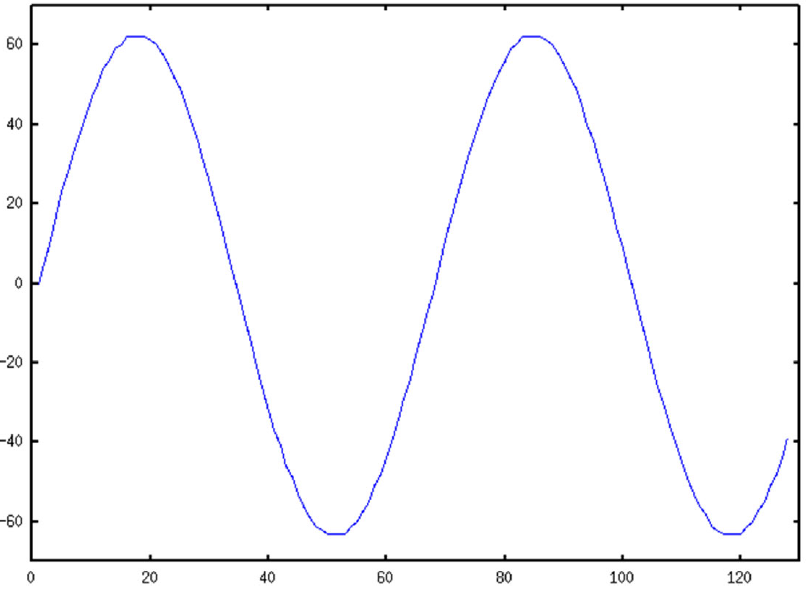
\includegraphics[width=0.8\textwidth]{images/Algoritmic_C/Figure_4_3.png}
			\caption{Rango máximo de un entero con signo de 7-bit}
		\end{figure}
		
	\end{frame}
	
	\begin{frame}
		\begin{figure}
			\centering
			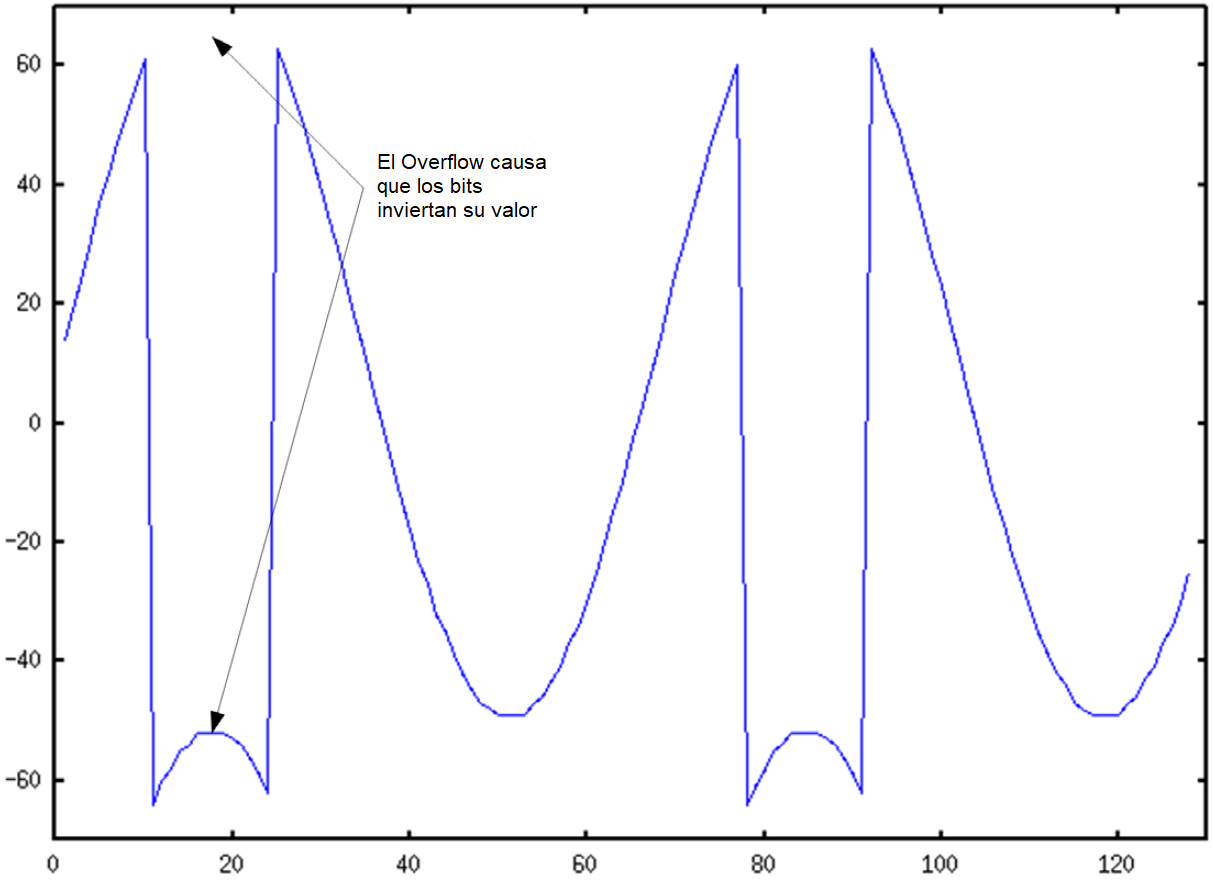
\includegraphics[width=0.8\textwidth]{images/Algoritmic_C/Figure_4_4.png}
			\caption{Efectos del wrapping en Tipos de datos con signo de 7-bit}
		\end{figure}
	\end{frame}


	\begin{frame}
	\justifying
	Los tipos de datos de punto fijo de Algorithmic C permiten a los diseñadores modelar un vector de bits con o sin signo con precisión de punto fijo estática. Esto es algo que no se puede hacer directamente en RTL y es una de las muchas ventajas de la síntesis de alto nivel. Aunque la mayoría de los algoritmos DSP se diseñan utilizando aritmética de punto flotante o fijo, la implementación RTL real se realiza con enteros, y el diseñador tiene que controlar manualmente el punto decimal desplazando los resultados intermedios a la izquierda o a la derecha. Este método de diseño no solo es tedioso, sino también propenso a errores. HLS permite a los diseñadores construir hardware directamente a partir de un modelo de punto fijo. Los tipos de datos \textbf{ac\_fixed} están estandarizados y permiten a los diseñadores especificar tanto el ancho entero como el fraccionario, así como el signo de las variables.
	\end{frame}
	
	\begin{frame}[fragile]{Tipos de datos de Punto Fijo sin signo}
	Los tipos de datos en punto fijo sin signo de Algorithmic C se declaran como:
	
	\begin{lstlisting}
		ac_fixed<W,I,false> x;
	\end{lstlisting}
	
	$0 <= x <= (1-2^W)2^I$ en incrementos de $2^{I-W}$\newline
	
	Se especifican tanto el ancho total \textbf{W} como el número de bits enteros \textbf{I}. Como resultado,  \textbf{I} determina la posición de la coma decimal con respecto al bit más significativo (MSB).
	
	\begin{figure}
		\centering
		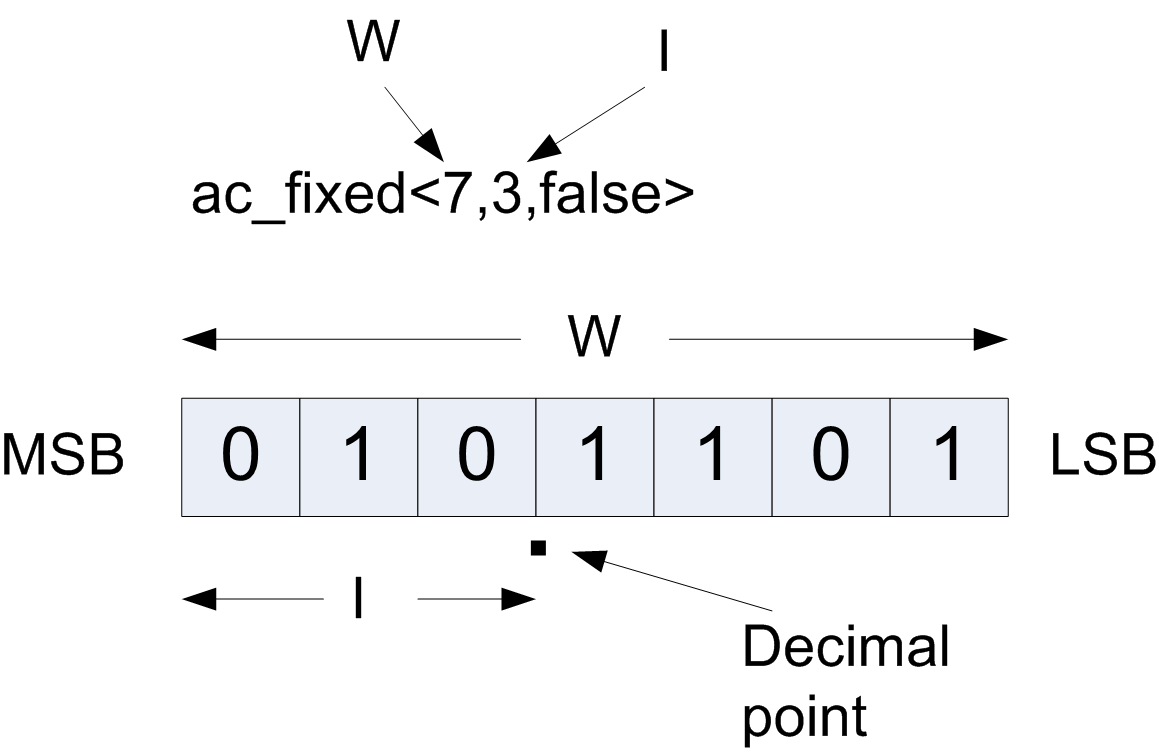
\includegraphics[width=0.38\textwidth]{images/Algoritmic_C/Figure_4_5.png}
		\caption{Posición del punto decimal en Punto Fijo}
	\end{figure}
	
	\note{Ahora que los tipos de datos de Algorithmic C permiten expresar valores fraccionarios, ya no es necesario escalar los resultados al dominio de los enteros. Tomando como ejemplo el Ejemplo 3, que escaló la onda sinusoidal para maximizar el rango dinámico del entero sin signo de 7 bits «x», y expresándola mediante tipos de datos de punto fijo sin signo, se obtiene el Ejemplo 5.}
	\end{frame}
	
	\begin{frame}[fragile]{Ejemplo 5 - Entero sin signo en punto fijo en Algorithmic C}
		\begin{lstlisting}
			#include <ac_fixed.h>
			#include <iostream.h>
			#include <fstream.h>
			#include <math.h>
			
			const double pi = 3.14;
			const double OFFSET = 1.0;
			
			int main(){
				fstream fptr;
				fptr.open("tmp.txt", fstream::out);
				ac_fixed<7,1,false> x[128];
				
				for(int i=0;i<128;i++){
					x[i] = OFFSET + 0.98*sin(2*pi*i/64);
					fptr << x[i] <<endl;
				}
				fptr.close();
			}
		\end{lstlisting}
	\note
	{
		Los detalles del Ejemplo 5 son:
		\begin{itemize}
			\item Line 1 includes the ac\_int library.
			\item Line 10 defines a 7-bit fixed point array “x” with one integer bit. This means that values of “x” can range somewhere between 0 and (1-2-7)*21 or 1.98. Supporting the full amplitude of the sine wave from -1 to 1 would require 2 integer bits.
			\item Line 13 computes the sine wave and adds an offset of one, keeping all values positive and preventing wrapping by keeping the amplitude of the sign wave from exceeding +/-0.98.
		\end{itemize}
	}
	\end{frame}
	
	\begin{frame}
	\begin{figure}
		\centering
		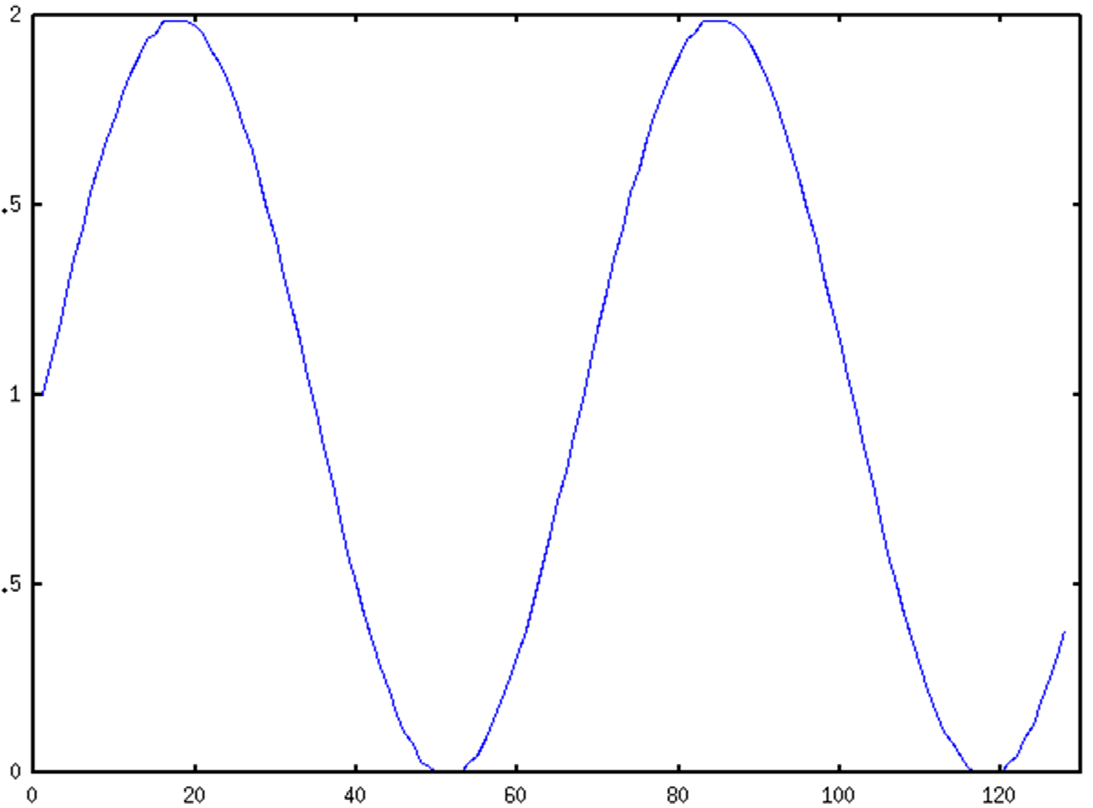
\includegraphics[width=0.8\textwidth]{images/Algoritmic_C/Figure_4_6.png}
		\caption{Señal senoidal con punto fijo sin signo de 7-bit}
	\end{figure}
		
	\end{frame}
		
	\begin{frame}[fragile]{Tipos de datos de Punto Fijo signado}
		Los tipos de datos en punto fijo sin signo de Algorithmic C se declaran como:
		
		\begin{lstlisting}
			ac_fixed<W,I,true> x;
		\end{lstlisting}
		
		$-0.5*2^I <= x <= (0.5*2^{-W})2^I$ en incrementos de $2^{I-W}$\newline
		
		\textbf{I} determina la ubicación del punto decimal en relación con el bit más significativo (MSB), que también es el bit de signo.
	
	\end{frame}
	
	\begin{frame}
		\begin{figure}
			\centering
			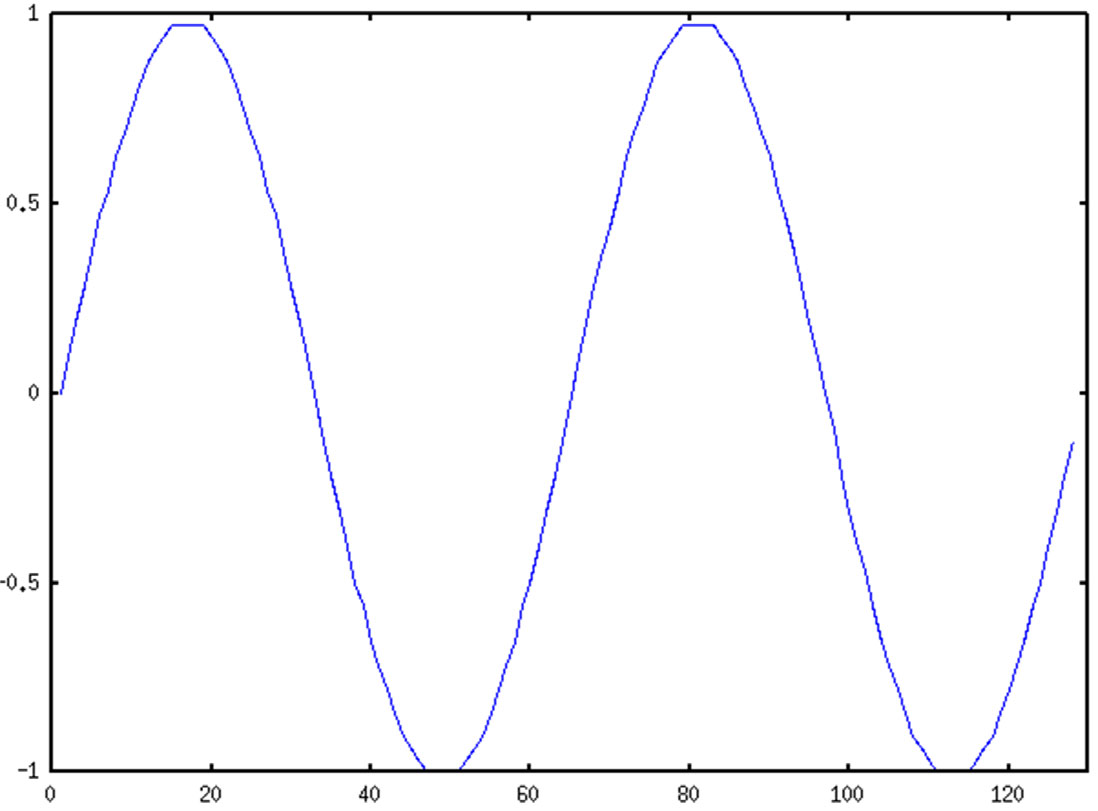
\includegraphics[width=0.8\textwidth]{images/Algoritmic_C/Figure_4_7.png}
			\caption{Señal senoidal en punto fijo con signo de 7-bit}
		\end{figure}
	\end{frame}
	
	\begin{frame}[fragile]{Cuantización y Overflow}
	\justifying
		Además de permitir expresar algoritmos de forma más natural, los tipos de datos de punto fijo también proporcionan mecanismos para gestionar la cuantización y el desbordamiento. El modo predeterminado de \textbf{'ac\_fixed'} consiste en truncar y desbordar, de forma similar a lo mostrado para \textbf{'ac\_int'}. Este modo no consume área adicional, pero puede no ser ideal para algunas aplicaciones. Los tipos de datos \textbf{ac\_fixed} admiten diversos modos de cuantización y desbordamiento, que se describen en detalle en el manual de tipos de datos de Algorithmic C. En este apartado se presentan las razones por las que podría ser conveniente habilitar estos modos. La cuantización y el desbordamiento se habilitan mediante parámetros de plantilla adicionales para los tipos de datos \textbf{'ac\_fixed'}.
		
		\begin{lstlisting}
		ac_fixed<W,I,S,Q,O> x;
		\end{lstlisting}
		
		donde \textbf{Q} y \textbf{O} setean los modos de quantización y overflow, respectivamente.
	\end{frame}
	
	
	\begin{frame}[fragile]{Truncado y Redondeo}
		\justifying
		El comportamiento predeterminado es truncar y descartar los bits a la derecha del bit menos significativo (LSB). Esto resulta en una pérdida total de información. Un ejemplo de esto sería asignar datos fraccionarios a una variable de punto fijo con solo bits enteros. Por ejemplo:
		
		\begin{lstlisting}
		ac_fixed<7,7,true> x = 0.5;
		\end{lstlisting}
		
		Al imprimir el valor de "x" después de la asignación, se obtiene cero, ya que "x" no contiene decimales. En lugar de descartar los decimales, se puede usar un modo de redondeo para redondear hacia arriba o hacia abajo según su valor. De forma similar a lo que aprendimos en la escuela primaria, podemos redondear hacia arriba o hacia abajo dependiendo de la posición del valor decimal entre dos números enteros.
		
		\begin{lstlisting}
		ac_fixed<7,7,true,AC_RND> x = 0.5;
		\end{lstlisting}
		
		\textbf{AC\_RND} redondea hacia el infinito positivo, lo que significa que a "x" se le asignará el valor de uno. El modo de redondeo redondea en función del incremento mínimo permitido definido por W e I.
	\end{frame}
	
	\begin{frame}{Saturación y Overflow}
	\justifying
	
	Los ejemplos anteriores mostraron que el comportamiento predeterminado es que los bits se "desborden" cuando se excede el valor máximo o mínimo representable. Esto se conoce como desbordamiento o subdesbordamiento y suele ser una situación muy indeseable. La mayoría de los algoritmos pueden, y deben, diseñarse para que el desbordamiento nunca ocurra. Esto implica tener en cuenta el rango dinámico de las variables y garantizar que el crecimiento interno de bits sea suficiente para representar todos los rangos posibles de entradas del algoritmo. Sin embargo, existen situaciones en las que es necesario garantizar que el desbordamiento nunca ocurra. Los sistemas de misión crítica, como el control de vuelo, serían un buen ejemplo donde el desbordamiento sería desastroso. Los algoritmos de vídeo son otro ejemplo de por qué el desbordamiento sería indeseable, ya que la mayoría de las personas no desean que los píxeles cambien de los colores más brillantes a los más oscuros.
	\end{frame}
	
	\begin{frame}{Saturación y Overflow}
	\justifying
	Se puede evitar el desbordamiento habilitando la saturación en el tipo de datos de punto fijo. Encontrará más detalles sobre el comportamiento de estos modos en el manual de tipos de datos de Algorithmic C. Se debe tener precaución al usar la saturación, ya que suele aumentar el área del diseño. NO habilite la saturación en todas las variables del diseño. La saturación se suele usar selectivamente en algunos lugares. El ejemplo 6 se ha reescrito para habilitar la saturación mediante el parámetro de plantilla de desbordamiento \textbf{AC\_SAT}, que se muestra en la línea 10 del ejemplo 7.\newline
		
	Tomando el Ejemplo 6 y agregando un pequeño desplazamiento positivo, el resultado se desbordará, lo que dará lugar a un resultado sin sentido o potencialmente catastrófico, como se muestra en la Figura 8.
	\end{frame}
	
	\begin{frame}
	\begin{figure}
		\centering
		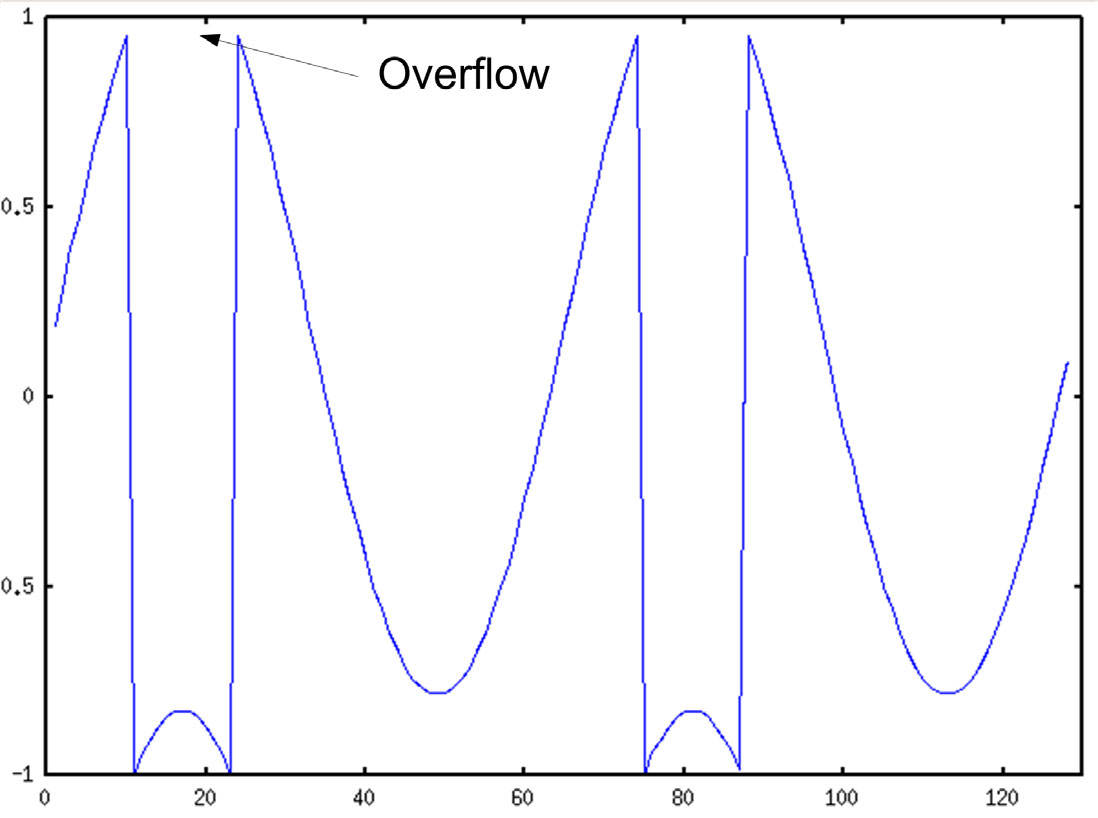
\includegraphics[width=0.8\textwidth]{images/Algoritmic_C/Figure_4_8.png}
		\caption{Overflow en punto fijo}
	\end{figure}
	\end{frame}
	
	\begin{frame}{Saturación y Overflow}
	\justifying
	Se puede evitar el desbordamiento habilitando la saturación en el tipo de datos de punto fijo. Encontrará más detalles sobre el comportamiento de estos modos en el manual de tipos de datos de Algorithmic C. Se debe tener precaución al usar la saturación, ya que suele aumentar el área del diseño. NO habilite la saturación en todas las variables del diseño. La saturación se suele usar selectivamente en algunos lugares. El ejemplo 6 se ha reescrito para habilitar la saturación mediante el parámetro de plantilla de desbordamiento \textbf{AC\_SAT}, que se muestra en la línea 10 del ejemplo 7.
	
	\end{frame}

	\begin{frame}[fragile]{Saturación y Overflow}
	
	\begin{lstlisting}
	#include <ac_fixed.h>
	#include <iostream.h>
	#include <fstream.h>
	#include <math.h>
	
	const double pi = 3.14;
	const double OFFSET = 0.2;
	
	int main(){
		fstream fptr;
		fptr.open("tmp.txt", fstream::out);
		ac_fixed<7,1,true,AC_TRN,AC_SAT> x[128];
		
		for(int i=0;i<128;i++){
			x[i] = OFFSET + 0.98*sin(2*pi*i/(double)64);
			fptr << x[i] <<endl;
			}
		fptr.close();
	}
	\end{lstlisting}
	
	\end{frame}

	\begin{frame}
		\begin{figure}
			\centering
			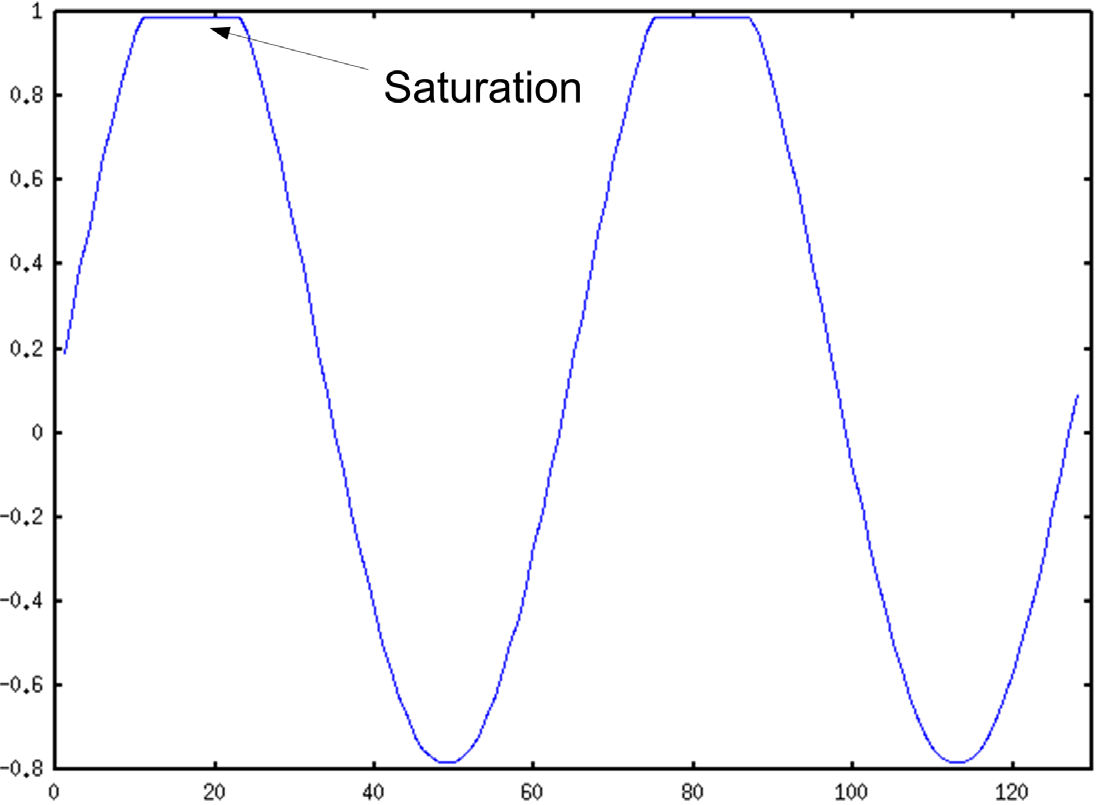
\includegraphics[width=0.6\textwidth]{images/Algoritmic_C/Figure_4_9.png}
			\caption{Efecto de Saturación}
		\end{figure}
	\note{		
	El análisis de la Figura 9 muestra que la habilitación de la saturación ha evitado cualquier desbordamiento o subdesbordamiento. Sin embargo, la figura también muestra claramente que la forma de onda es no lineal. Esta no linealidad, también conocida como recorte, introduce ruido en el sistema. Esta es una de las principales razones por las que la mayoría de los algoritmos deben diseñarse sin utilizar la saturación.
	}
	
	\footnotesize \justifying
	La saturación solo debe usarse cuando sea absolutamente necesario. La mayoría de los algoritmos pueden diseñarse para evitar el desbordamiento/subdesbordamiento seleccionando los anchos de bits variables adecuados para admitir el rango dinámico completo del algoritmo. La saturación suele afectar tanto al área como al rendimiento.
	\end{frame}
	
	\begin{frame}{Operadores}
	\justifying \footnotesize
	Todos los operadores aritméticos y lógicos estándar de C++ son compatibles con los tipos de datos \textbf{ac\_int} y \textbf{ac\_fixed}. Operadores como la multiplicación y la suma están diseñados para devolver un resultado sin pérdida de precisión. Para una descripción completa de todos los operadores, consulte el manual de referencia de Algorithmic C.\\Operadores como la división (``/'') y el módulo (``\%'') son compatibles, pero deben usarse con precaución cuando los operandos son variables. Esto se debe a que una operación como la división consume mucha memoria, y la mayoría de los diseñadores de hardware no utilizan divisores de memoria. Este es un aspecto de HLS que suele malinterpretarse, ya que es perfectamente razonable escribir algo como 'z = x/y' en C++. Si realmente se necesita una división, existen implementaciones más eficientes, como el algoritmo CORDIC. La mayoría de las herramientas de HLS proporcionan una biblioteca que implementa estas funciones de forma más eficiente. Las divisiones o el módulo por una constante son mucho más aceptables y se implementan mediante lógica de suma y desplazamiento. La división o el módulo por una potencia de dos se implementan mediante desplazamientos estáticos, sin coste adicional de área. Dos operadores cuyo comportamiento merece mención son la selección de bits y el desplazamiento, pero primero, un breve repaso de los operadores aritméticos.
	\end{frame}
	
	
	\begin{frame}[fragile]{Operadores aritméticos Bitwise: *, +, -, /, \&, |, \textasciicircum,\%}
		\justifying \small
	Los operadores aritméticos bit a bit de Algorithmic C están diseñados para que no haya pérdida de precisión en el valor de retorno. Además, se admite la combinación de tipos de datos con y sin signo de Algorithmic C, y se devuelve el signo esperado.	\\
	El tipo de retorno de una operación aritmética gestiona automáticamente el crecimiento de bits para evitar la pérdida de precisión. Esto se logra automáticamente porque el ancho de bits de los dos operandos se especifica como parámetros de template al declarar las variables \textbf{ac\_int}. Esto se muestra a continuación:
		
	\begin{lstlisting}
	ac_int<8,true> a,b; 	//8-bits signado	
	\end{lstlisting}
	Multiplicando ``a'' por ``b'', cada uno con precisión de 8 bits, requieres 16 bits de precisión:
	\begin{lstlisting}
		(returns ac_int<16,true>)(a*b)
	\end{lstlisting}
	La suma ``a'' + ``b'' requiere 9 bits de precisión:
	\begin{lstlisting}
		(returns ac_int<9,true>)(a+b)
	\end{lstlisting} 
		
	\end{frame}
	
	
	\begin{frame}[fragile]{Operador selector de Bit: \textbf{[]}}
	\justifying \footnotesize
	Se pueden leer o escribir bits individuales de un tipo de datos \textbf{ac\_int} o  \textbf{ac\_fixed} mediante el operador \textbf{[]}. El índice del operador selecciona la posición del bit; por ejemplo, `x[1]`, `x[3]`, `x[7]`. El valor devuelto es un objeto de la clase \textbf{ac\_int::bitref} y se proporciona una función de conversión integrada a \textbf{ac\_int} y \textbf{bool}. El siguiente fragmento de código muestra cómo se puede usar el operador de selección de bits para leer el bit de signo de un \textbf{ac\_int}.	
		
	\begin{lstlisting}
	ac_int<11,true> x;
	bool is_neg;
	
	if(x[10]) //test for sign bit treated as bool
		is_neg = true;
	else
		is_neg = false;
	\end{lstlisting}
	El operador de selección de bit se puede usar con la misma facilidad para escribir un bit en un \textbf{ac\_int} o \textbf{ac\_fixed}. Por ejemplo: 
	\begin{lstlisting}
	ac_fixed<9,1,false> x = 0;
	bool add_one = true;
	
	if(add_one)
		x[8] = 1; 	//set MSB of x
	\end{lstlisting}
	\end{frame}

	\begin{frame}{Operadores de desplazamiento: \textbf{<<}, \textbf{>>}}
	\justifying \footnotesize
	Los operadores de desplazamiento merecen un análisis detallado porque, a diferencia de los operadores aritméticos que mantienen la precisión completa, devuelven la precisión del operando izquierdo. Esto puede generar resultados inesperados. Además, los diseñadores deben prestar atención a cómo utilizan los desplazamientos, ya que ambos operandos pueden ser con o sin signo. Esto también puede dar lugar a resultados sorprendentes que no serían posibles en RTL tradicional.
	\end{frame}

	\begin{frame}[fragile]{Desplazamiento a la derecha sin signo: \textbf{>>}}
	\justifying \footnotesize
	El operador de desplazamiento a la derecha sin signo, aplicado a los tipos de datos \textbf{ac\_int} o \textbf{ac\_fixed} sin signo, se comporta exactamente como un diseñador RTL esperaría de un desplazador. Cada bit se desplaza a la derecha la cantidad de desplazamiento y se insertan ceros en los bits más significativos. 
	\note{Esto se aprecia mejor en el ejemplo gráfico de la Figura 10. La variable que se desplaza es un entero sin signo de 4 bits inicializado con todos sus bits a 1. A medida que aumenta la cantidad de desplazamiento, se insertan ceros en los bits más significativos.}
	
	\begin{lstlisting}
	ac_int<4,false> x = -1; //set all bits to 1's
	int idx;
	ac_int<4,false> y = x >> idx;	
	\end{lstlisting}
	
	\begin{figure}
	\centering
	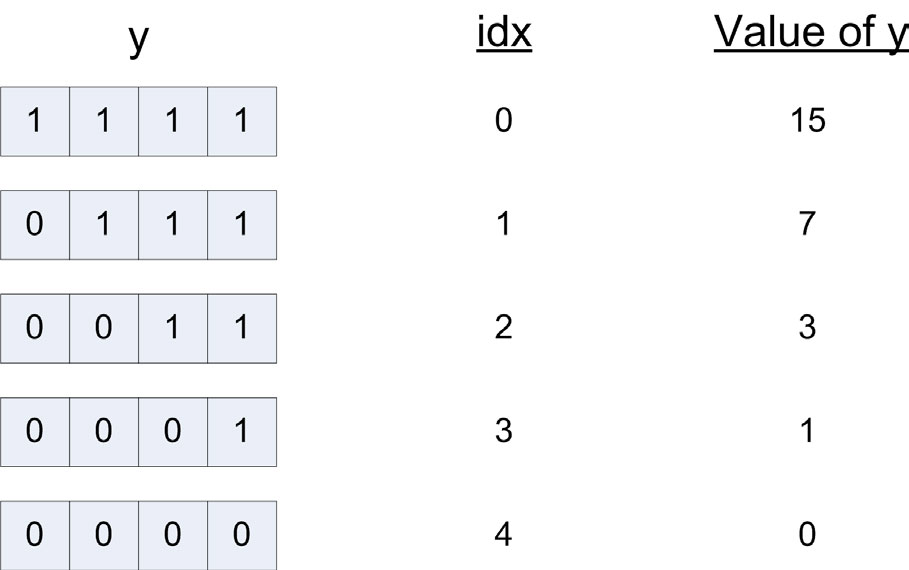
\includegraphics[width=0.5\textwidth]{images/Algoritmic_C/Figure_4_10.png}
	\caption{Desplazamiento a la derecha de números sin signo}
	\end{figure}
	
	\end{frame}
	
	\begin{frame}[fragile]{Desplazamiento a la derecha con signo: \textbf{>>}}
	\justifying \footnotesize
	El desplazamiento a la derecha con signo tiene un comportamiento algo inesperado. \note{La mayoría de los ingenieros de hardware consideran los desplazamientos a la derecha y a la izquierda como divisiones o multiplicaciones por potencias de dos. Por lo tanto, cabría esperar que, en algún punto, el desplazamiento a la derecha pusiera todos los bits a cero, como se muestra en la Figura 10. Sin embargo,} Al desplazar a la derecha un \textbf{ac\_int} con signo, el bit de signo siempre se conserva, lo que tiene como resultado final el desplazamiento de unos desde el bit más significativo (MSB) en lugar de ceros. 
	\note{Esto se muestra en la Figura 11. El \textbf{ac\_int} "x" se inicializa con el bit de signo igual a uno y todos los demás bits a cero, lo que equivale a menos ocho. Cada desplazamiento creciente tiene el efecto de dividir por potencias de dos crecientes hasta que todos los bits se establecen en uno. A partir de este punto, el resultado siempre es negativo uno.}
	
	\begin{lstlisting}
	ac_int<4,true> x = 0;
	x[3] = 1 	//set x equal -8
	int idx;
	ac_int<4,true> y = x >> idx;	
	\end{lstlisting}
	
	\begin{figure}
	\centering
	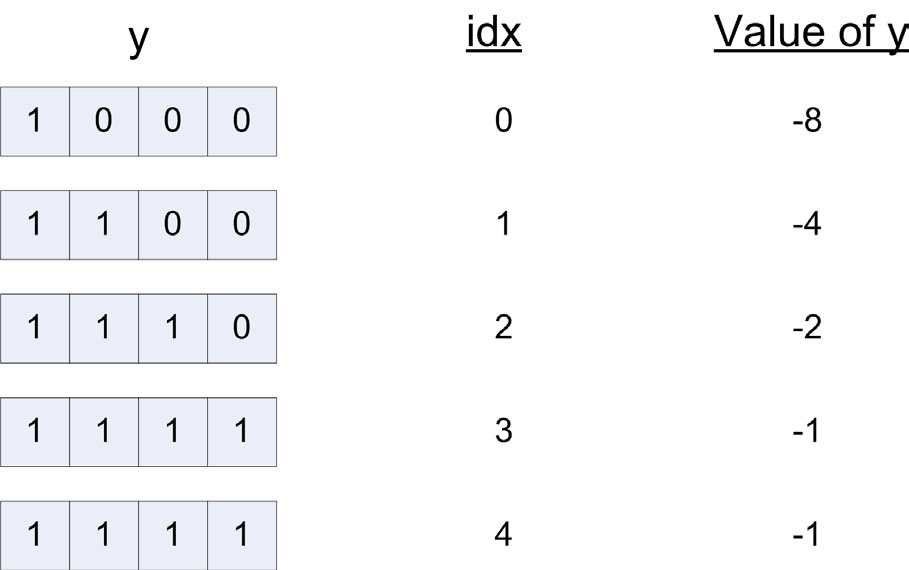
\includegraphics[width=0.5\textwidth]{images/Algoritmic_C/Figure_4_11.png}
	\caption{Desplazamiento a la derecha de números con signo}
	\end{figure}
		
	\end{frame}
	
	
	\begin{frame}[fragile]{Desplazamiento a la izquierda sin signo: \textbf{<<}}
	\justifying \footnotesize
	Desplazar un entero sin signo \textbf{ac\_int} a la izquierda y asignar el resultado a una variable con la misma precisión tiene un comportamiento similar al de un desplazamiento sin signo a la derecha, excepto que se insertan ceros desde la posición del bit menos significativo (LSB).
	\begin{lstlisting}
	ac_int<4,false> x = -1; //set all bits to 1's
	int idx;
	ac_int<4,false> y = x << idx;		
	\end{lstlisting}
	
	\begin{figure}
		\centering
		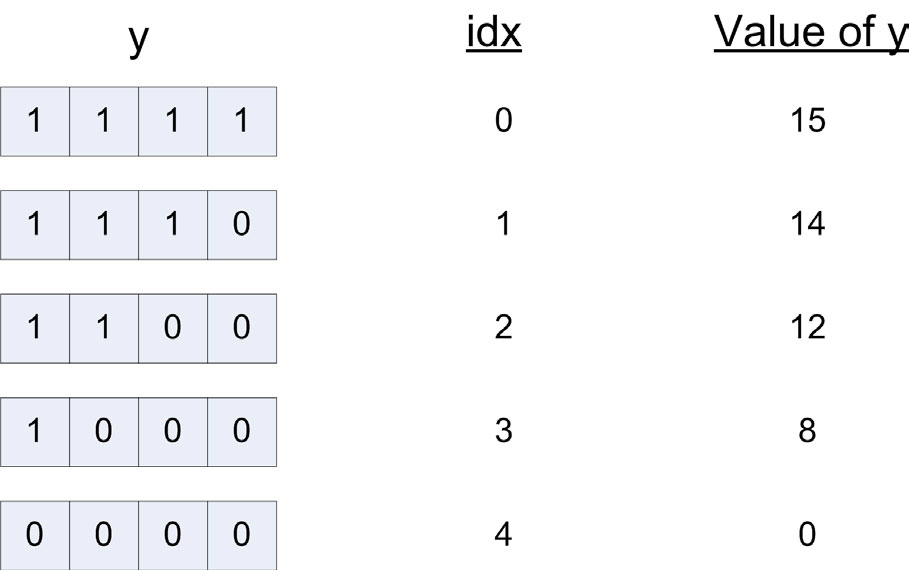
\includegraphics[width=0.5\textwidth]{images/Algoritmic_C/Figure_4_12.png}
		\caption{Desplazamiento a la izquierda de números sin signo}
	\end{figure}
	\end{frame}
	
	\begin{frame}[fragile]{Desplazamiento a la izquierda con signo: \textbf{<<}}
	\justifying \footnotesize
	El desplazamiento a la izquierda con signo tiene un comportamiento similar al desplazamiento a la izquierda sin signo, donde se insertan ceros desde el bit menos significativo (LSB).
	\begin{lstlisting}
	ac_int<4,true> x = -1; //set all bits to 1's
	int idx;
	ac_int<4,true> y = x << idx;	
	\end{lstlisting}
	
	\begin{figure}
	\centering
	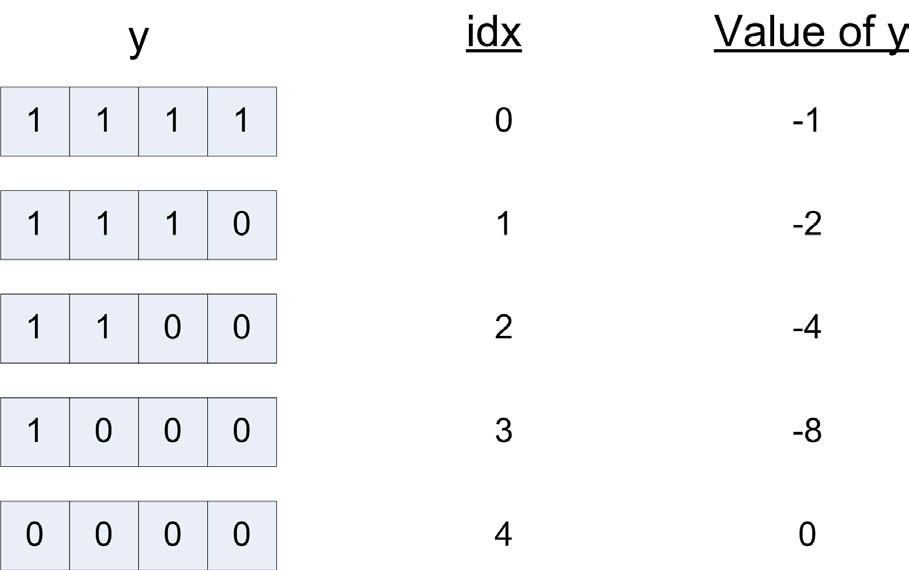
\includegraphics[width=0.5\textwidth]{images/Algoritmic_C/Figure_4_13.png}
	\caption{Desplazamiento a la izquierda de números con signo}
	\end{figure}
	\end{frame}
	
	
	
	\begin{frame}[fragile]{Pérdida inesperada de precisión}
	\justifying \footnotesize
	El desplazamiento a la izquierda puede tener un comportamiento inesperado, pero correcto, cuando se espera que el resultado se base en la precisión de las variables objetivo. Esto se entiende mejor viendo un ejemplo:
	\begin{lstlisting}
	ac_int<4,false> x = -1; 	//set all bits to 1's
	int idx;
	ac_int<8,false> y = x << idx;
	\end{lstlisting}
	
	En el ejemplo anterior, ``x'', un valor de cuatro bits sin signo, se desplaza a la izquierda y se asigna a ``y'', un valor de ocho bits sin signo. Un error común entre los diseñadores que se inician en los tipos de datos de Algorithmic C es creer que los bits más significativos de ``x'' se almacenan en ``y'' al desplazarse más allá del bit más significativo (MSB) de ``x''. La figura 14 muestra el comportamiento real. Recuerde que el operador de desplazamiento devuelve la precisión del operando izquierdo, que en este ejemplo es de cuatro bits. Para conservar los bits que se desplazan más allá del MSB de ``x'', es necesario convertir ``x'' a la precisión de ``y''. Por ejemplo:
	\begin{lstlisting}
	ac_int<4,false> x = -1; 	//set all bits to 1's
	int idx;
	ac_int<8,false> y = (ac_int<8,false>) x << idx;
	\end{lstlisting}
	\end{frame}
	
	
	\begin{frame}[fragile]{Pérdida inesperada de precisión}
	\justifying \footnotesize
	\begin{framed}
	El desplazamiento a la izquierda puede provocar la pérdida de bits si la variable que se está desplazando no tiene la misma precisión que la parte izquierda de la asignación.	
	\end{framed}
	
	Esto ahora da el comportamiento deseado que se muestra en la Figura 15.	

		
	\begin{figure}
	\centering
	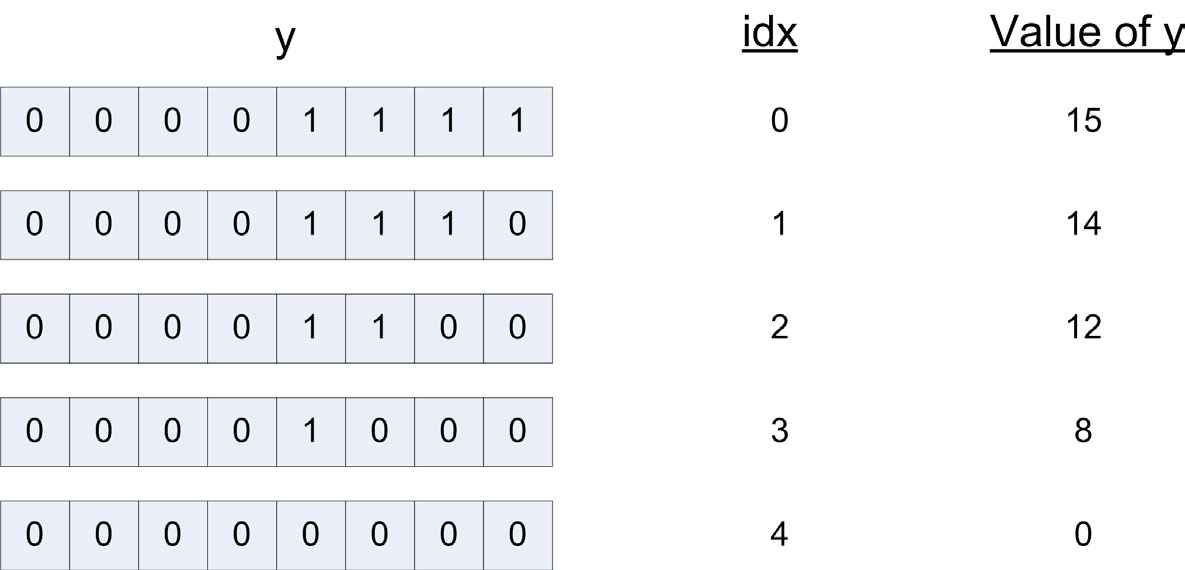
\includegraphics[width=0.7\textwidth]{images/Algoritmic_C/Figure_4_14.png}
	\caption{Pérdida inesperada de precisión cuando se desplaza a la izquierda}
	\end{figure}
	\end{frame}
	
	\begin{frame}[fragile]{Pérdida inesperada de precisión}
	\justifying \footnotesize
	
	\begin{figure}
		\centering
		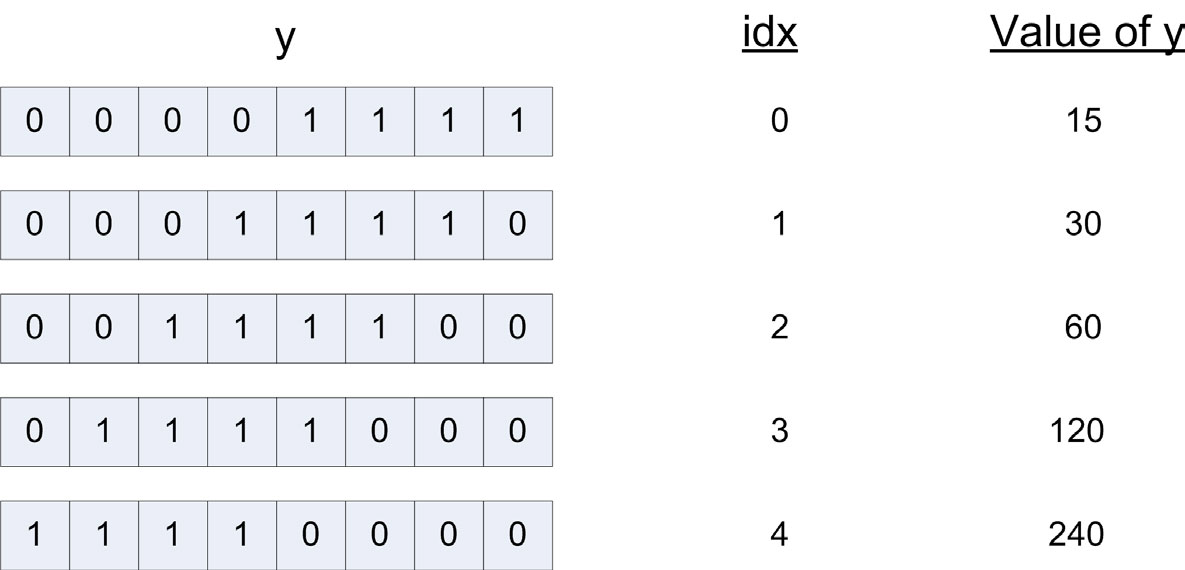
\includegraphics[width=0.7\textwidth]{images/Algoritmic_C/Figure_4_15.png}
		\caption{Casteado a la precisión deseada cuando se desplaza a la izquierda}
	\end{figure}
		
	\end{frame}
	
	\begin{frame}{Métodos}
	Los tipos de datos de Algorithmic C proporcionan varios métodos integrados que se describen en detalle en el manual de referencia. \newline
	
	\url{https://hlslibs.org/}\newline
	
	Los métodos más utilizados para el diseño y la simulación se describen a continuación.
	\end{frame}	
	
	\begin{frame}[fragile]{Slice Read: slc}
	\justifying \footnotesize
	El método de lectura de segmento tiene la forma: $slc<W>(int lsb)$ \newline
	
	Donde el parámetro de plantilla ``W'' especifica el ancho del segmento, y ``lsb'' indica dónde comienza el segmento. No es posible ajustar dinámicamente el ancho del segmento porque ``W'' es un parámetro de plantilla. Sin embargo, sí es posible cambiar dinámicamente el valor de ``lsb''. Considere el siguiente ejemplo donde se lee un segmento de tres bits de ``x'' y se asigna a ``y''. ``lsb'' apunta a la posición del bit dos. La figura muestra gráficamente cómo funciona la lectura del segmento. \\
	\begin{lstlisting}
	ac_int<8,false> x = 100;
	ac_int<3,false> y;
	
	y = x.slc<3>(2);	
	\end{lstlisting}
	
	\end{frame}
	
	\begin{frame}[fragile]{Slice Read: slc}
	\justifying \footnotesize
	El método de lectura de segmento tiene la forma: $slc<W>(int lsb)$ \newline
	
	\begin{figure}
		\centering
		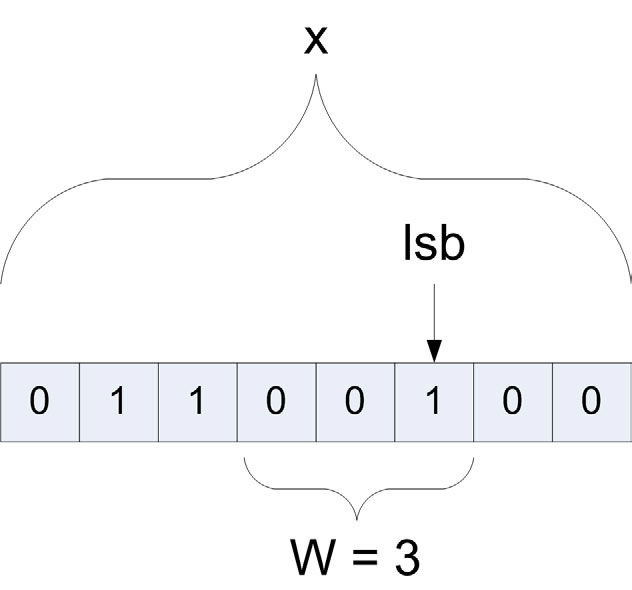
\includegraphics[width=0.5\textwidth]{images/Algoritmic_C/Figure_4_16.png}
		\caption{Lectura de segmento}
	\end{figure}
	\end{frame}
	
	\begin{frame}[fragile]{Problemas con la compilación del método Read Slice}
	\justifying \footnotesize
	Algunos compiladores pueden generar errores cuando se utiliza el método \textbf{read slice} dentro de una función o clase con plantillas. Si esto ocurre, simplemente coloque la palabra clave \textbf{template} antes del nombre del método.\newline
	\begin{lstlisting}
		ac_int<8,false> x = 100;
		ac_int<3,false> y;
		
		y = x.template slc<3>(2);	
	\end{lstlisting}
	\end{frame}
	
	\begin{frame}[fragile]{Slice Write: set\_slc}
	\justifying \footnotesize
	El método \textbf{set\_slc} tiene la forma: \textbf{set\_slc(int lsb, const ac\_int<W,S> \&slc)}\newline
	\\Donde \textbf{lsb} es el índice del vector de bits e indica dónde se debe escribir el segmento. Este comportamiento es esencialmente el mismo que el mostrado para las lecturas de segmentos en la Figura 16. El segmento que se escribe puede ser un entero con o sin signo (\textbf{ac\_int}). Al igual que con las lecturas de segmentos, el tamaño del segmento no se puede modificar dinámicamente. Su uso es el siguiente:\newline
	\begin{lstlisting}
	ac_int<8,false> x = 0;
	ac_int<3,false> y = 5;
	
	x.set_slc(2,y);	
	\end{lstlisting}
	\end{frame}
	
	\begin{frame}[fragile]{Funciones de conversión explícitas}
	\justifying \footnotesize
	Los tipos de datos de Algorithmic C proporcionan varias funciones de conversión implícitas y explícitas. Estas se encuentran completamente documentadas en el manual de referencia del lenguaje. Las funciones de conversión explícitas suelen ser necesarias al asignar un \textbf{ac\_fixed} a un \textbf{ac\_int}, o al intentar usar \textbf{printf} para imprimir los resultados de una simulación. El primer caso genera un error de compilación, y el segundo, al usar  \textbf{printf}, provoca un error de segmentación en tiempo de ejecución.
	\begin{lstlisting}
	ac_fixed<8,3,false> x = 3.185;
	ac_int<8,false> y;
	\end{lstlisting}
	
	El asignamiento que aparece a continuación genera un error de compilación.
	\begin{lstlisting}
	y = x;
	\end{lstlisting}
	
	Debería escribirse
	\begin{lstlisting}
	y = x.to_int();
	\end{lstlisting}
	
	La siguiente instrucción provoca un error de segmentación en tiempo de ejecución:
	\begin{lstlisting}
	printf("%d\n",y);
	\end{lstlisting}
	Debería escribirse
	\begin{lstlisting}
	printf("%d\n",y.to_int());
	\end{lstlisting}
	
	\end{frame}

	\begin{frame}[fragile]{Funciones de conversión implícitas}
	\justifying \footnotesize
	Los tipos de datos de algorithmic C tienen funciones de conversión integradas para el operador de asignación ``='' hasta 64 bits. Estas funciones convierten automáticamente los tipos de datos algorithmic C de vuelta a tipos nativos. Esto permite usar variables directamente para comprobar condicionalmente cualquier bit activado en el vector de bits. Por ejemplo:
	\begin{lstlisting}
	ac_int<64,false> ctrl = 37;
	if(ctrl)	//test for any bit set to a one
		tmp += din;
	\end{lstlisting}
		
	\begin{framed}
	Un error de compilación ocurre si ``ctrl'' es mayor que 64 bits. En este caso, debe utilizarse una de las funciones de conversión explícitas.
	\end{framed}
	\end{frame}
	
	\begin{frame}{Funciones de Ayuda/Útiles}
	Las librerías Algorithmic C proveen algunas funciones útiles para el diseño de hardware.
	\end{frame}
	
	\begin{frame}[fragile]{Array Uninitialization: ac::init\_array}
		\justifying \footnotesize
		Esta función permite inicializar y desinicializar un array con una constante o un valor irrelevante. La ventaja de usar esta función integrada es que la herramienta HLS puede optimizar el array de forma más eficiente, ya que no necesita analizar bucles ni asignaciones para determinar la intención. El uso más común de esta función es desinicializarlo, es decir, asignar valores irrelevantes a todos sus elementos. Esto se hace para evitar que el hardware borre todas las ubicaciones de un array estático mapeado en memoria. Por definición en el lenguaje C++, una variable declarada como estática se inicializa a cero al ser creada. En muchos casos, no es necesario liberar la memoria de un diseño, ya que se sabe que la memoria se escribe antes de leerse. De este modo, se puede eliminar la sobrecarga de recorrer inicialmente cada ubicación de memoria. La función \textbf{ac::init\_array} tiene la siguiente forma:
		\begin{lstlisting}
		bool ac::init_array<"init value">("base address of array", "number of elements");
		\end{lstlisting}
		Considere el siguiente fragmento de código donde la matriz ``a'' se asigna a una memoria.
		
		\begin{lstlisting}
		static int a[1000];
		static bool dummy = ac::init_array<AC_VAL_DC>(a,1000);
		\end{lstlisting}
		
		\note{La razón por la que se utiliza ``dummy'' y se declara estático es que solo queremos llamar a la función \textbf{init\_array} una vez durante la inicialización.}
	\end{frame}
	
	\begin{frame}[fragile]{ceil, floor, y nbits}
	\justifying \footnotesize
	A menudo es necesario calcular estáticamente el número mínimo de bits requeridos para un tipo de datos de Algorithmic C con el fin de indexar una matriz. Se proporcionan las siguientes funciones:
	\begin{itemize}
		\item ac::log2\_ceil<x>::val - returns the number of bits required to index ``x'' elements.
		\item ac::log2\_floor<x>::val - returns log2(x).
		\item ac::nbits<x>::val - returns number of bits required to represent ``x''.
	\end{itemize}
	En todos estos casos, ``x'' debe ser estáticamente determinable. Por ejemplo:
	\begin{lstlisting}
	const int WORDS = 175;
	void foo(int data[WORDS],
	ac_int<ac::log2_ceil<WORDS>::val,false> idx,
	int &dout){
		dout = data[idx];
	}
	\end{lstlisting}
	En el ejemplo anterior, ``idx'' se ha definido con el número mínimo de bits necesarios para indexar los elementos ``WORDS''.
	\end{frame}
	
	\begin{frame}{Tipos de Datos Complejos}
	Las bibliotecas de tipos de datos de precisión de bits de Algorithmic C también admiten tipos de datos complejos, lo que elimina la necesidad de que los diseñadores desarrollen sus propias clases complejas. El tipo de datos \textbf{ac\_complex} es una clase con plantillas que se puede usar con \textbf{ac\_int} y \textbf{ac\_fixed}, así como con tipos nativos de C++. Para obtener información sobre su uso y restricciones, consulte el manual de tipos de datos de Algorithmic C.
	\end{frame}

	\begin{frame}{Referencias}
	\begin{itemize}
		\item High-Level Synthesis Blue Book -  Michael Fingeroff (2010) Ed. Xlibris Us
		\item \url{https://hlslibs.org/}
		\item \url{http://www.mentor.com/products/esl/high_level_synthesis/ac_datatypes}
	\end{itemize}
	\end{frame}
	
	\begin{frame}
	\centering
	\Huge \textbf{Q\&A}
	\end{frame}

%		\begin{frame}[fragile]{}
	%		
	%		
	%		\begin{lstlisting}
		%			#include <ac_int.h>
		%			#include <ac_fixed.h>
		%		\end{lstlisting}
	%		\newline
	%		
	%		
	%	\end{frame}
%	



%		\begin{frame}[fragile]{}
	%		
	%		
	%		\begin{lstlisting}
		%			#include <ac_int.h>
		%			#include <ac_fixed.h>
		%		\end{lstlisting}
	%		\newline
	%		
	%		
	%	\end{frame}
%	


%		\begin{frame}[fragile]{}
	%		
	%		
	%		\begin{lstlisting}
		%			#include <ac_int.h>
		%			#include <ac_fixed.h>
		%		\end{lstlisting}
	%		\newline
	%		
	%		
	%	\end{frame}
%	


%		\begin{frame}[fragile]{}
	%		
	%		
	%		\begin{lstlisting}
		%			#include <ac_int.h>
		%			#include <ac_fixed.h>
		%		\end{lstlisting}
	%		\newline
	%		
	%		
	%	\end{frame}
%	



%		\begin{frame}[fragile]{}
	%		
	%		
	%		\begin{lstlisting}
		%			#include <ac_int.h>
		%			#include <ac_fixed.h>
		%		\end{lstlisting}
	%		\newline
	%		
	%		
	%	\end{frame}
%	


%		\begin{frame}[fragile]{}
	%		
	%		
	%		\begin{lstlisting}
		%			#include <ac_int.h>
		%			#include <ac_fixed.h>
		%		\end{lstlisting}
	%		\newline
	%		
	%		
	%	\end{frame}
%	



%		\begin{frame}[fragile]{}
	%		
	%		
	%		\begin{lstlisting}
		%			#include <ac_int.h>
		%			#include <ac_fixed.h>
		%		\end{lstlisting}
	%		\newline
	%		
	%		
	%	\end{frame}
%	

%		\begin{frame}[fragile]{}
	%		
	%		
	%		\begin{lstlisting}
		%			#include <ac_int.h>
		%			#include <ac_fixed.h>
		%		\end{lstlisting}
	%		\newline
	%		
	%		
	%	\end{frame}
%	
	
	
	
	
	
	
	
\end{document}